\begin{document}
\title{COMS3008A Assignment -- Report}
\author{Sayfullah Jumoorty, 2430888}
\date{\today}
\maketitle 
%\thispagestyle{empty}
\pagestyle{fancy}
\fancyhf{}
\fancyhead[R]{\thepage}
\fancyhead[L]{COMS3008A Assinment}
%\vskip 3mm 
%\pagenumbering{roman}
%\newpage
\pagenumbering{arabic} 

\section{Problem 1: Parallel Scan}
In computer science, a scan operation, also known as a prefix sum operation, is a common parallel algorithm used to compute a cumulative sum or other associative operation on a sequence of elements. The result of the scan operation is a new sequence where each element represents the accumulation of values up to that point in the original sequence.

\subsection{Test Data Generation}
In order to get accurate results, it is important to have an efficient data generation technique for huge sets of random numbers, and also, an efficient storage type to quickly read the data between programs:

\textbf{Input:} An integer exponent $n$.

\textbf{Output:} A binary file containing a sequence of random integers.

\begin{enumerate}
    \item Read the integer exponent $n$ from the command-line arguments.
    \item Check if the number of arguments is valid. If not, print an error message and exit.
    \item Convert the exponent $n$ to an integer.
    \item Check if $n$ is a non-negative number. If not, print an error message and exit.
    \item Calculate the size of the array as $2^n$. This determines the number of integers to be generated.
    \item Allocate memory for an array of integers with the calculated size.
    \item Create a random number generator using the Mersenne Twister engine, seeded with the current system clock time.
    \item Define a uniform integer distribution that generates random numbers between a specified range.
    \item Iterate from 0 to the size of the array, assigning each element a random number generated by the distribution.
    \item Open a binary output file for writing.
    \item Write the content of the array to the output file as a sequence of bytes.
    \item Free the memory allocated for the array.
    \item Exit the program with a success status code.
\end{enumerate}

\subsection{Serial Implementation}
As we are tying to get the most optimal base line algorithm, we can hence do the following for the serial program:

\begin{itemize}
    \item Read the input array from a binary file.
    \item Check if the size of the input array is a power of two.
    \item The prefix sum calculation is performed using the scan function. The function takes the input array (nums) and produces the prefix sum array \lstinline|(prefix_sum)| using a simple for loop algorithm. Each element in the prefix sum array is computed by adding the corresponding element in the input array to the sum of all previous elements. This process can be seen in $Algorithm 1$
\end{itemize}

The serial approach performs all these steps sequentially, without parallelization. It serves as a baseline for performance comparison and is suitable for situations where parallelization is not required or feasible due to hardware or software limitations. The serial approach can be used for small input sizes or when the overhead of parallelization outweighs the benefits.
\\ \\

\begin{figure}[htb]
    \begin{minipage}{0.5\textwidth}
        \begin{algorithm}[H]
            \SetKwFunction{scan}{scan}
            \SetKwProg{Fn}{Function}{}{}
            
            \Fn{\scan{$\text{out}: \text{vector}[\text{int}], \text{in}: \text{vector}[\text{int}]$}}{
                $N \gets \text{in.size()}$\;
                $\text{out.resize}(N)$\;
                
                \If{$N > 0$}{
                    $\text{out}[0] \gets \text{in}[0]$\;
                }
                
                \For{$i \gets 1$ \KwTo $N-1$}{
                    $\text{out}[i] \gets \text{in}[i] + \text{out}[i - 1]$\;
                }
            }
            \caption{Scan function}
        \end{algorithm}
    \end{minipage}%
    \begin{minipage}{0.5\textwidth}
        \centering
        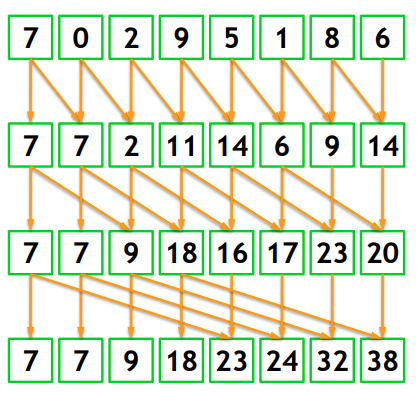
\includegraphics[width=0.7\linewidth]{pics/scanExample.png}
        \caption{Process of Scan}
        \label{fig:scanExample}
    \end{minipage}
\end{figure}

\newpage

\subsection{OpenMP Implementation}
In the OpenMP version of the code, several changes were made to parallelize the computation using OpenMP directives. This included using a scan method known as "Blelloch" \cite{blelloch1990prefix}. The algorithm for scan operation in $Algoritm 1$ is inherently sequential, as there is a loop carried dependence in the for loop. However, Blelloch 1990 gives an algorithm for calculating the scan operation in parallel. Here is a clear explanation of the approach, parallelization methods, correctness, and testing methods:

\begin{enumerate}
  \item \textbf{Parallelization Approach:}
  \begin{itemize}
    \item The code uses the OpenMP library to introduce parallelism and exploit multiple threads to speed up the computation.
    \item Parallelization is applied to the "Up-sweep (reduce)" and "Down-sweep (scan)" phases of the Blelloch scan algorithm.

    \begin{itemize}
    \item Perform the up-sweep (reduce) phase of the Blelloch scan algorithm:
    \begin{itemize}
        \item Starting with a stride $d$ of 1, iterate over the array.
        \item Perform the reduction operation by adding each element at index $i + d - 1$ to the element at index $i + 2 \cdot d - 1$.
        \item Repeat the process for increasing values of $d$ until it reaches the array size.
        \item Store the last value of the up-sweep phase.
    \end{itemize}
    \item Set the root of the binary tree to zero by modifying the last element of the array.
    \item Perform the down-sweep (scan) phase of the Blelloch scan algorithm:
    \begin{itemize}
        \item Starting with a stride $d$ equal to half the array size, iterate over the array.
        \item Perform the scan operation by swapping and accumulating the elements.
        \item Repeat the process for decreasing values of $d$ until it reaches 1.
    \end{itemize}
    \item Adjust the array size to accommodate the additional element and set the last element to the value obtained from the up-sweep phase.
    \item Compute the prefix sum array.
    \end{itemize}
    
  \end{itemize}

  \item \textbf{Parallelization Methods:}
  \begin{itemize}
    \item The parallelization \cite{parallelalgorithms} is achieved using OpenMP directives, which control the distribution of work among multiple threads.
    \item The following OpenMP directives are used in the code:
    \begin{itemize}
      \item \lstinline|#pragma omp parallel| creates a team of threads.
      \item \lstinline|#pragma omp for| distributes the loop iterations among the threads.
      \item \lstinline|#pragma omp single| ensures that a particular section of code is executed by only one thread.
    \end{itemize}
  \end{itemize}

  \newpage

  \item \textbf{Up-sweep (Reduce) Phase:}
  \begin{itemize}
    \item The up-sweep phase is parallelized using the OpenMP directive \lstinline|#pragma omp for|.
    \item The loop that performs the reduction operation is divided among multiple threads, with each thread handling a subset of the iterations.
    \item The \lstinline|reduction(+ : last)| clause is used to perform a reduction operation on the \lstinline|last| variable, ensuring that each thread contributes its local sum to the final value.
  \end{itemize}

  \begin{figure}[htb]
	\centering
	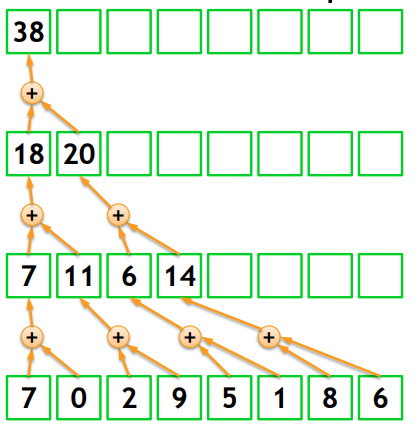
\includegraphics[width=0.3\linewidth]{pics/scanUpSweep.png}
    	\caption{Up-sweep (Reduce) Phase}\label{fig:scanExample}
\end{figure}

  \item \textbf{Down-sweep (Scan) Phase:}
  \begin{itemize}
    \item The down-sweep phase is parallelized using the OpenMP directive \lstinline|#pragma omp parallel for|.
    \item Similar to the up-sweep phase, the loop is divided among multiple threads, allowing them to work on different subsets of the iterations.
  \end{itemize}

  \begin{figure}[htb]
	\centering
	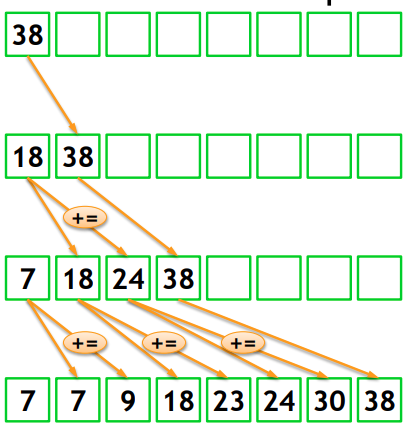
\includegraphics[width=0.3\linewidth]{pics/scanDownSweep.png}
    	\caption{Down-sweep (Scan) Phase}\label{fig:scanDownSweep}
\end{figure}

  \begin{center}
    \begin{algorithm}[H]
        \SetKwFunction{blellochscan}{blelloch_scan}
        \SetKwProg{Fn}{Function}{}{}
        
        \Fn{\blellochscan{$\text{nums}: \text{vector}[\text{int}]$}}{
            $n \gets \text{nums.size()}$\;
            
            \tcp{Up-sweep (reduce) phase}
            $last \gets 0$\;
            \#pragma omp parallel default(none) shared(nums, n) reduction(+ : last)\;
            \{
                \For{$d \gets 1$ \KwTo $n-1$ step $2*d$}{
                    \#pragma omp for\;
                    \For{$i \gets 0$ \KwTo $n-1$ step $2*d$}{
                        $\text{nums}[i + 2 * d - 1] += \text{nums}[i + d - 1]$\;
                    }
                }
                \#pragma omp single\;
                {
                    $last \gets \text{nums}[n - 1]$\;
                }
            \}
            
            \tcp{Set root to 0}
            $\text{nums}[n - 1] \gets 0$\;
            
            \tcp{Down-sweep (scan) phase}
            \For{$d \gets n / 2$ \KwTo $1$ step $d / 2$}{
                \#pragma omp parallel for\;
                \For{$i \gets 0$ \KwTo $n-1$ step $2*d$}{
                    $t \gets \text{nums}[i + d - 1]$\;
                    $\text{nums}[i + d - 1] \gets \text{nums}[i + 2 * d - 1]$\;
                    $\text{nums}[i + 2 * d - 1] += t$\;
                }
            }
            
            \tcp{Increase the size of the array by 1 and set the last element to the last value of the up-sweep phase}
            $\text{nums.resize}(n + 1)$\;
            $\text{nums}[n] \gets last$\;
            
            \tcp{Remove the first element of the array}
            $\text{nums.erase}(\text{nums.begin}())$\;
        }
        
        \caption{Blelloch scan function}
    \end{algorithm}
\end{center}

  \item \textbf{Correctness:}
  \begin{itemize}
    \item The correctness of the prefix sum computation is ensured by validating the result against a temporary array using the \lstinline|validatePrefixSum| function.
    \item The function checks if the prefix sum values in the final array match the expected values based on the original array.
    \item If a mismatch is found, the program terminates with an error message indicating that the prefix sum is invalid.
  \end{itemize}

  \item \textbf{Testing Methods:}
  \begin{itemize}
    \item The code includes a \lstinline|checkIfPowerOfTwo| function to verify if the size of the input array is a power of two.
    \item This check is important because the Blelloch scan algorithm assumes a power-of-two input size.
    \item If the size is not a power of two, the program terminates with an error message.
  \end{itemize}
\end{enumerate}

\subsection{Graph Comparison - OpenMP}
The scalability can be evaluated by varying the input size or the number of threads (t) and observing the impact on execution time. In the provided results, the execution time decreases as the number of processing elements increases (t=2 to t=8). This suggests that the code exhibits reasonable scalability, as distributing the workload among more threads leads to faster execution times.

\begin{figure}[htb]
	\centering
	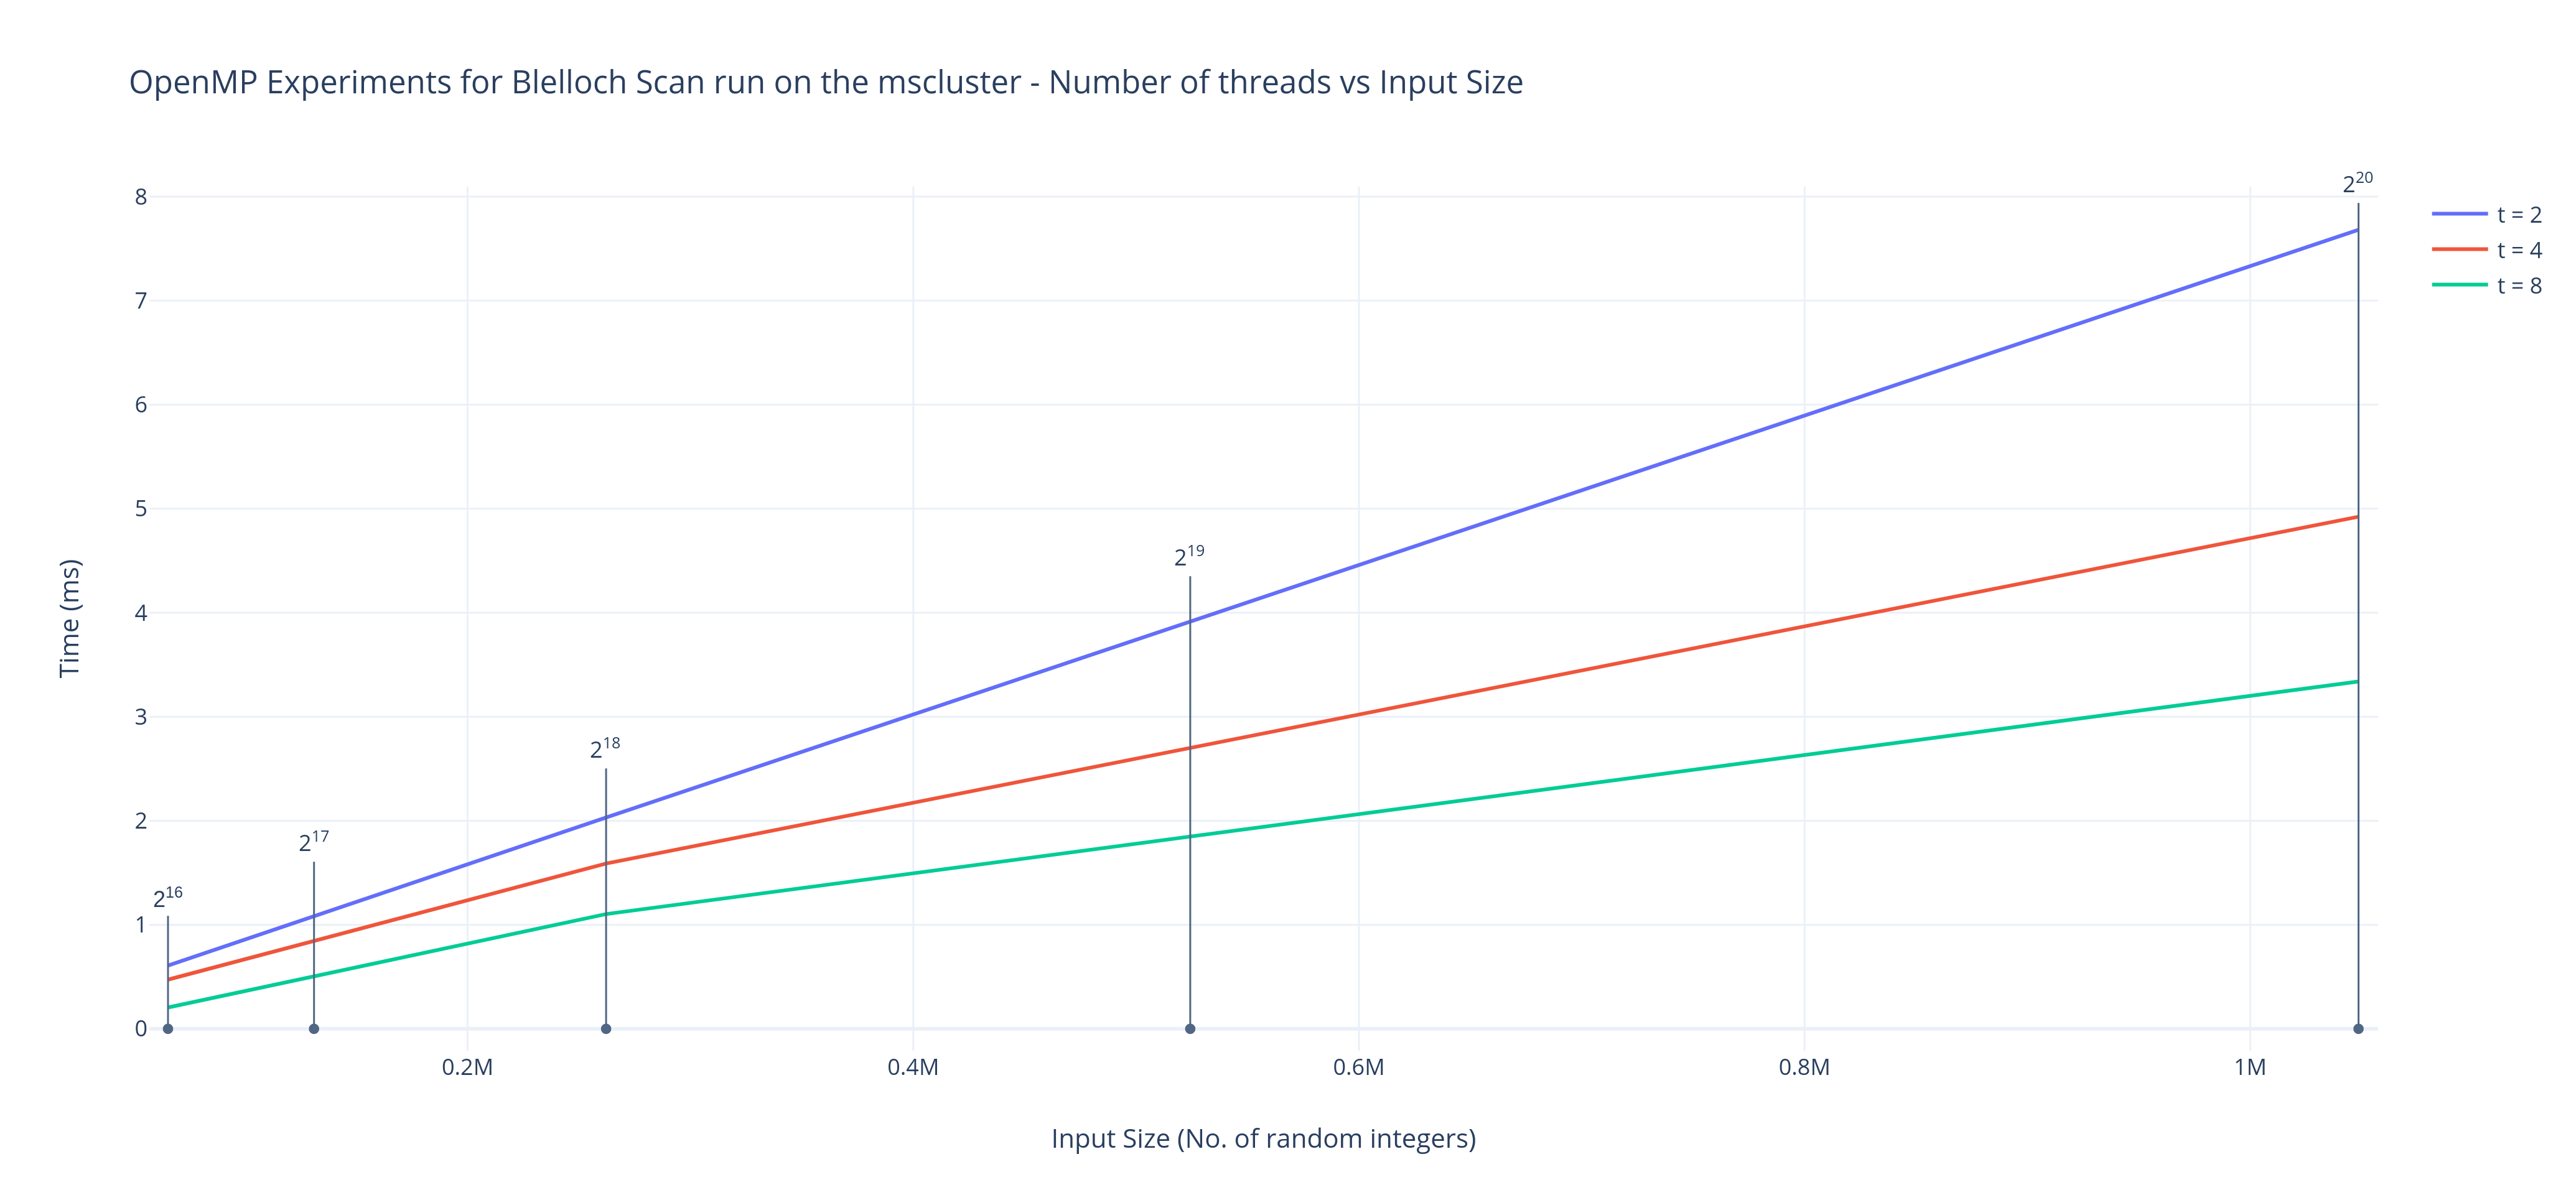
\includegraphics[width=0.8\linewidth]{pics/ompScan.png}
    	\caption{OpenMP Comparisons for blelloch scan}\label{fig:ompScan}
\end{figure}

From the graph, we can see a direct relation to increasing the number of threads for different input sizes results in a speedup, and that speedup gets significantly better as the input size grows.

\subsection{MPI Implementation}
In the MPI \cite{mpi} implementation of the code, we know solve the computation using the Message Passing Interface (MPI) library.

\begin{enumerate}
  \item \textbf{Parallelization Approach:}
  \begin{itemize}
    \item The code uses the MPI library to distribute the work among multiple processes and enable communication between them.
    \item Parallelization is achieved by dividing the input data and computations among different MPI processes.
  \end{itemize}

  \item \textbf{Parallelization Methods:}
  \begin{itemize}
    \item The MPI library provides various functions for process management, communication, and collective operations.
    \item The code utilizes MPI functions such as \lstinline{MPI_Init}, \lstinline{MPI_Comm_size}, \lstinline{MPI_Comm_rank}, \lstinline{MPI_Bcast}, \lstinline{MPI_Scatter}, \lstinline{MPI_Gather}, and \lstinline{MPI_Finalize} to achieve parallelization and coordination among processes.
  \end{itemize}

  \item \textbf{Differences from Serial and OpenMP Approaches:}
  \begin{itemize}
    \item Unlike the serial approach, where the computation is performed sequentially on a single thread, and the OpenMP approach, which parallelizes the computation using multiple threads within a shared memory environment, the MPI approach distributes the computation across multiple processes running on separate memory spaces.
    \item In the MPI implementation, each process works on a subset of the input data and performs computations independently. Communication between processes is necessary to exchange data and synchronize the results.
    \item MPI allows scaling the computation across multiple machines, making it suitable for distributed memory systems, clusters, or supercomputers.
  \end{itemize}

  \item \textbf{Approach to Solving the Problems:}
  \begin{itemize}
    \item The input data is read from a binary file and stored in a vector on the root process (rank 0).
    \item The size of each chunk of data is calculated on the root process and broadcasted to all other processes using \lstinline{MPI_Bcast}.
    \item The input data is then scattered among the processes using \lstinline{MPI_Scatter}.
    \item Each process performs the prefix sum computation on its local input data using the Blelloch scan algorithm, similar to the serial and OpenMP approaches.
    \item Global sums are gathered from each process to the root process using \lstinline{MPI_Gather}.
    \item The root process performs the Blelloch scan on the gathered global sums.
    \item Each process receives a single global sum and adds it to its local input data.
    \item Finally, the modified local input data is gathered from each process to the root process, resulting in the final prefix sum array.
  \end{itemize}

  \item \textbf{Correctness:}
  \begin{itemize}
    \item The correctness of the prefix sum computation is ensured by validating the result against the original input data using the \lstinline{validatePrefixSum} function.
    \item The function checks if the prefix sum values in the final array match the expected values based on the input data.
    \item If any mismatch is found, an error message is printed, and the program is aborted using \lstinline{MPI_Abort}.
  \end{itemize}

  \item \textbf{Testing Methods:}
  \begin{itemize}
    \item The code measures the time taken to perform the prefix sum computation using \lstinline{MPI_Wtime}.
    \item The time is printed and saved to a CSV file for analysis.
    \item Additionally, the correctness of the prefix sum is validated using \lstinline{validatePrefixSum}.
    \item The testing methods can include running the code on different input sizes, comparing the results with the sequential and OpenMP implementations, and evaluating the performance scalability with an increasing number of MPI processes.
  \end{itemize}
\end{enumerate}

\subsection{Performance Evaluation}
To evaluate the performance of the baseline (serial) version compared to the parallel version and test the scalability by varying the number of processing elements, we can analyze the provided results. We can a generalized discussion of the performance evaluation, in which results were obtained by running the different implementations on the mscluster using 4 nodes with 4 processes each, and with an input size of $2^{n}$ random integers:

\subsection*{Comparison of Performance (Speedup) - Serial vs. OpenMP}

\begin{table}[htbp]
  \caption{Comparison of Performance (Speedup) - Serial vs. OpenMP}
  \centering
  \begin{tabular}{lcc}
    \toprule
    \textbf{Description} & \textbf{Time (ms)} & \textbf{Speedup} \\
    \midrule
    Serial Time & 18.9288 ms & -- \\
    Parallel Time & 7.36385 ms & 2.57 \\
    \bottomrule
  \end{tabular}
\end{table}

The table above compares the execution time of the serial version and the parallel version of the code. The "Serial Time" represents the time taken by the code in the serial execution mode. The "Parallel Time" represents the time taken by the code when parallelized. The "Speedup" column indicates the speedup achieved by the parallel version compared to the serial version. In this case, the parallel version achieved a speedup of 2.57, indicating that the parallel implementation is 2.57 times faster than the serial implementation.

\subsection*{Comparison of Performance (Speedup) - Serial vs. MPI Version}

\begin{table}[htbp]
  \caption{Comparison of Performance (Speedup) - Serial vs. MPI Version}
  \centering
  \begin{tabular}{lcc}
    \toprule
    \textbf{Description} & \textbf{Time (ms)} & \textbf{Speedup} \\
    \midrule
    Serial Time & 18.9288 ms & -- \\
    MPI Time (np=4) & 8.47074 ms & 2.23 \\
    \bottomrule
  \end{tabular}
\end{table}

The table above compares the execution time of the serial version and the MPI version of the code. The "Serial Time" represents the time taken by the code in the serial execution mode. The "MPI Time (np=4)" represents the time taken by the code when parallelized using MPI with 4 processing elements. The "Speedup" column indicates the speedup achieved by the MPI version compared to the serial version. In this case, the MPI version achieved a speedup of 2.23, indicating that the MPI implementation with 4 processing elements is 2.23 times faster than the serial implementation.

\subsection*{Testing Scalability - Varying the Input Size or Number of Processing Elements}

\begin{table}[htbp]
  \caption{Testing Scalability - Varying the Input Size or Number of Processing Elements}
  \centering
  \begin{tabular}{lcc}
    \toprule
    \textbf{Description} & \textbf{Time (ms)} & \textbf{Speedup} \\
    \midrule
    $2^{16}$ & 1.80664 ms & 1.03 \\
    $2^{18}$ & 4.30736 ms & 1.74 \\
    $2^{20}$ & 8.47074 ms & 2.23 \\
    \bottomrule
  \end{tabular}
\end{table}

The table above shows the execution times and speedup for different input sizes or number of processing elements. In this case, the input size was varied while keeping the number of processing elements fixed at 4. The "Speedup" column indicates the speedup achieved by the parallel MPI version compared to the serial version. As the input size increased from $2^{16}$ to $2^{20}$, the speedup also increased from 1.03 to 2.23, indicating that the code exhibits good scalability.

Overall, the parallel version (using either OpenMP or MPI) outperforms the serial version in terms of speedup, demonstrating the benefits of parallelization. The MPI version shows improvements compared to the serial version, indicating the effectiveness of MPI parallelization. Furthermore, the code exhibits good scalability by achieving faster execution times as the input size increases. Further scalability analysis can be performed by varying the input size or number of processing elements in future evaluations.

\subsection{Graph Comparison - MPI}
The scalability can be evaluated by varying the input size or the number of processing elements (np) and observing the impact on execution time. In the provided results, the execution time decreases as the number of processing elements increases (np=2 to np=4). This suggests that the code exhibits reasonable scalability, as distributing the workload among more processes leads to faster execution times.

\begin{figure}[htb]
	\centering
	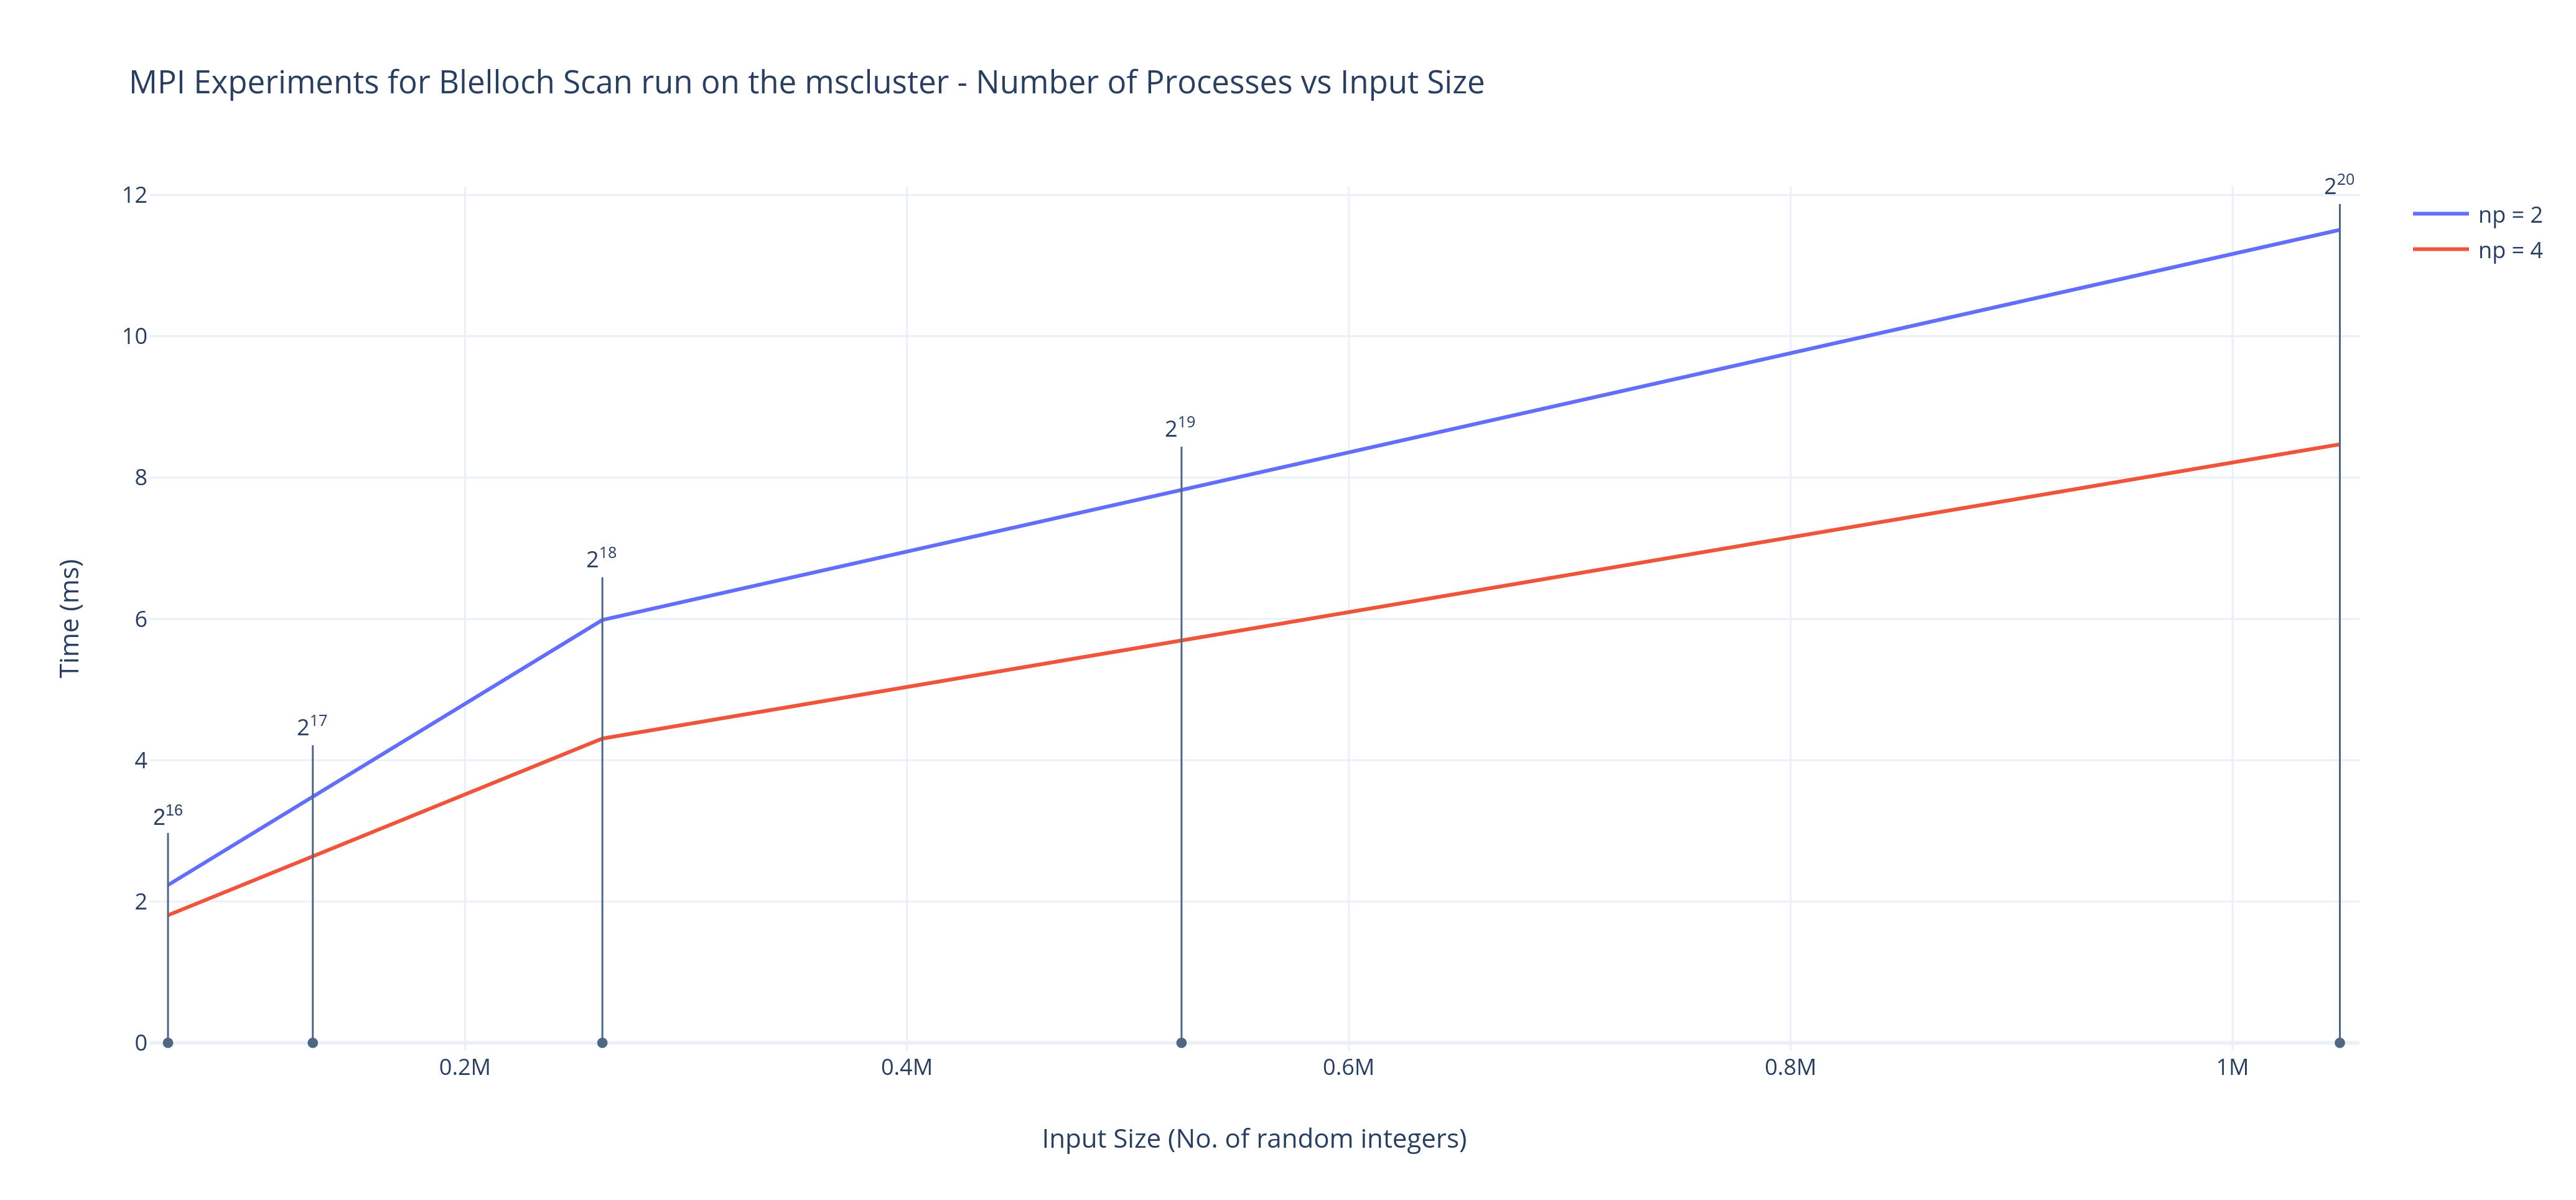
\includegraphics[width=0.9\linewidth]{pics/MPIGraphScan.png}
    	\caption{MPI Comparisons for blelloch scan}\label{fig:MPIGraphScan}
\end{figure}

From the graph, we can see a direct relation to increasing the number of processes for different input sizes results in a speedup, and that speedup gets significantly better as the input size grows.

\newpage

\section{Problem 2: Parallel Bitonic Sort}

\begin{itemize}
\item The \textbf{bitonic sort} algorithm is based on the concept of a \textbf{sorting network}.
\item This algorithm is particularly \textbf{well-suited for parallel processing}, making it a popular choice for sorting on \textbf{Graphics Processing Units (GPUs)}.
\item It \textbf{efficiently sorts} a given list or array of elements in ascending or descending order.
\end{itemize}

\subsection{Test Data Generation}
The method mentioned in $1.1$ is also used for generation of data for the various bitonic approaches, in order to get valuable and meaningful results.

\subsection{Serial Implementation}
In order to solve the problem of sorting in a bitonic \cite{bitonic1980} manner, we can break it apart and think of it as sections:

\begin{itemize}
  \item \textbf{Bitonic Sequence Validation}:
  \begin{itemize}
    \item The input sequence is checked to determine if it is a valid bitonic sequence.
    \item A bitonic sequence is defined as a sequence of numbers that first increases and then decreases (or vice versa).
    \item The program compares each element in the sequence with its adjacent element and checks if the order is consistent with the desired direction.
    \item If the order is violated at any point, an error message is displayed, indicating that the sequence is not a valid bitonic sequence.
  \end{itemize}
  
  \item \textbf{Power of Two Check}:
  \begin{itemize}
    \item The size of the input vector is checked to ensure that it is a power of two.
    \item A power of two is a number that can be expressed as $2^n$, where $n$ is a non-negative integer.
    \item This check is performed to ensure that the sorting algorithm works correctly.
    \item If the size of the input vector is not a power of two, it indicates an invalid input, and the program exits.
  \end{itemize}

  \newpage
  
  \item \textbf{Bitonic Merge}:
  \begin{itemize}
    \item The bitonic merge operation is a key step in the Bitonic Sort algorithm.
    \item It merges two sorted sequences in a bitonic manner, resulting in a sequence that is either strictly increasing or strictly decreasing.
    \item The algorithm compares the elements at corresponding positions in both sequences and swaps them if they violate the desired order.
    \item This process is repeated recursively until the entire sequence is merged.
  \end{itemize}

  \begin{center}
    \begin{algorithm}[H]
        \SetKwFunction{bitonicmerge}{bitonicMerge}
        \SetKwProg{Fn}{Function}{}{}
        
        \Fn{\bitonicmerge{$\text{arr}: \text{vector}[\text{int}], \text{low}: \text{int}, \text{cnt}: \text{int}, \text{direction}: \text{bool}$}}{
            \If{$\text{cnt} > 1$}{
                $k \gets \text{cnt} / 2$\;
                \For{$i \gets \text{low}$ \KwTo $\text{low} + k - 1$}{
                    \If{$\text{direction} = (\text{arr}[i] > \text{arr}[i + k])$}{
                        \text{swap}($\text{arr}[i]$, $\text{arr}[i + k]$)\;
                    }
                }
                \bitonicmerge($\text{arr}, \text{low}, k, \text{direction}$)\;
                \bitonicmerge($\text{arr}, \text{low} + k, k, \text{direction}$)\;
            }
        }
        
        \caption{Bitonic merge function}
    \end{algorithm}
\end{center}
  
  \item \textbf{Bitonic Sort}:
  \begin{itemize}
    \item The Bitonic Sort algorithm is based on the concept of bitonic sequences and bitonic merge.
    \item It recursively divides the input sequence into two halves, sorts each half independently in a bitonic manner, and then performs bitonic merge operations to merge the sorted halves.
    \item This process is repeated until the entire sequence is sorted in the desired order.
  \end{itemize}

  \begin{center}
    \begin{algorithm}[H]
        \SetKwFunction{bitonicsort}{bitonicSort}
        \SetKwProg{Fn}{Function}{}{}
        
        \Fn{\bitonicsort{$\text{numbers}: \text{vector}[\text{int}], \text{left}: \text{size\_t}, \text{size}: \text{size\_t}$}}{
            $\text{groupSize} \gets 2$\;
            $\text{itr} \gets \log_2(\text{size})$\;
            $\text{increasing} \gets \text{true}$\;
            
            \For{$i \gets 0$ \KwTo $\text{itr} - 1$}{
                \For{$j \gets 0$ \KwTo $\text{size} - 1$ step $\text{groupSize}$}{
                    $\text{increasing} \gets ((j / \text{groupSize}) \mod 2 = 0)$\;
                    \text{bitonicMerge}($\text{numbers}, \text{left} + j, \text{groupSize}, \text{increasing}$)\;
                }
                $\text{groupSize} \gets \text{groupSize} \times 2$\;
            }
        }
        
        \caption{Bitonic sort function}
    \end{algorithm}
\end{center}

\newpage
  
  \item \textbf{Testing and Timing}:
  \begin{itemize}
    \item The main function of the program handles the input and output operations.
    \item It reads a sequence of numbers from a file, performs the bitonic sort algorithm on the sequence, and measures the execution time.
    \item The sorted sequence is validated to ensure that it is a valid bitonic sequence.
    \item The execution time is recorded and saved to a file for further analysis.
  \end{itemize}
\end{itemize}

The correctness of the approach can be evaluated through rigorous testing, including unit tests, integration tests, boundary tests, and performance tests. These tests cover various scenarios and inputs to ensure that the code functions correctly and produces accurate results.

\begin{figure}[htb]
	\centering
	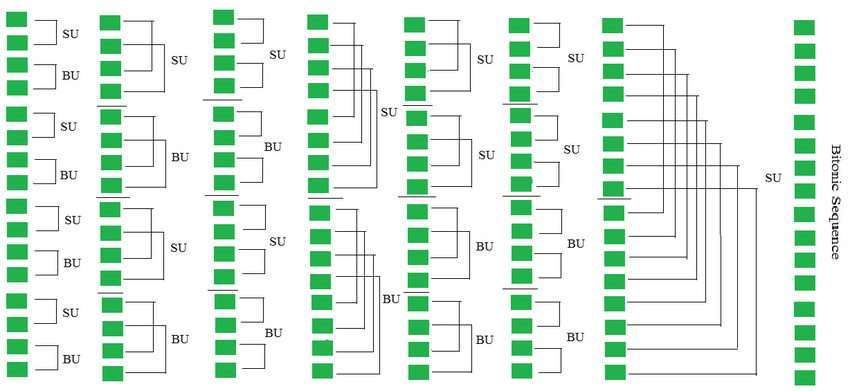
\includegraphics[width=0.8\linewidth]{pics/bitonicExample.png}
    	\caption{Bitonic Sequence}\label{fig:scanDownSweep}
\end{figure}

\newpage

\subsection{OpenMP Implementation}

\textbf{Parallelization Approach:}

The parallelization \cite{parallelalgorithms} approach in the code aims to improve the performance of the bitonic sort algorithm by utilizing parallel execution of sorting operations. Parallelization involves dividing the workload among multiple threads to execute tasks concurrently. This approach takes advantage of the parallel processing capabilities of modern multi-core or multi-processor systems to speed up the sorting process.

\textbf{Parallelization Methods:}

\begin{enumerate}
\item \textbf{Parallel For Loop:} The main parallelization method used in the code is the \lstinline|#pragma omp parallel for| directive. It parallelizes the outer loop in the \texttt{bitonicSort} function, which iterates over different group sizes. By adding this directive, the iterations of the loop are distributed among multiple threads, allowing them to work on different parts of the sequence concurrently. This parallelization method effectively divides the workload and reduces the overall execution time.

\item \textbf{Private Variables:} To ensure data integrity and prevent data races, the \texttt{private(increasing)} clause is added to the parallel for loop directive. This makes each thread have its private copy of the \texttt{increasing} variable, which is used within the loop. By making the variable private to each thread, conflicts that may occur during concurrent execution are avoided.
\end{enumerate}

\begin{figure}[htb]
    \begin{minipage}{0.5\textwidth}
        \begin{center}
            \begin{algorithm}[H]
                \SetKwFunction{bitonicsort}{bitonicSort}
                \SetKwProg{Fn}{Function}{}{}
                
                \Fn{\bitonicsort{$\text{numbers}: \text{vector}[\text{int}], \text{left}: \text{size\_t}, \text{size}: \text{size\_t}$}}{
                    $\text{groupSize} \gets 2$\;
                    $\text{itr} \gets \log_2(\text{size})$\;
                    $\text{increasing} \gets \text{true}$\;
                    
                    \For{$i \gets 0$ \KwTo $\text{itr} - 1$}{
                        \#pragma omp parallel for private(increasing)\;
                        \For{$j \gets 0$ \KwTo $\text{size} - 1$ step $\text{groupSize}$}{
                            $\text{increasing} \gets ((j / \text{groupSize}) \mod 2 = 0)$\;
                            \text{bitonicMerge}($\text{numbers}, \text{left} + j, \text{groupSize}, \text{increasing}$)\;
                        }
                        $\text{groupSize} \gets \text{groupSize} \times 2$\;
                    }
                }
                
                \caption{OpenMP Bitonic sort function}
            \end{algorithm}
        \end{center}
    \end{minipage}%
    \begin{minipage}{0.5\textwidth}
        \centering
        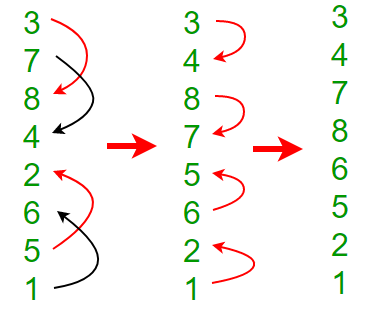
\includegraphics[width=0.7\linewidth]{pics/bitonicSteps.png}
        \caption{Sort Method}
        \label{fig:bitonicSteps}
    \end{minipage}
\end{figure}

\newpage

\textbf{Correctness and Testing Methods:}

To ensure the correctness of the parallelized approach, rigorous testing methods can be employed. This includes:

\begin{enumerate}
\item \textbf{Functional Testing:} Test the sorting algorithm with various inputs, including different bitonic sequences, to verify that the parallelized code produces the expected sorted output. This testing should cover both ascending and descending order sequences.

\item \textbf{Validation Testing:} Validate the sorted sequence to ensure that it is a valid bitonic sequence. Compare the sorted sequence with the original input sequence and check if it satisfies the bitonic property (either strictly increasing or strictly decreasing). This validation step ensures the correctness of the sorting algorithm.

\item \textbf{Boundary Testing:} Test the parallel code with edge cases and boundary conditions, such as small input sizes, large input sizes, and extreme values. This helps identify any potential issues or limitations of the parallelization approach.

\item \textbf{Performance Testing:} Measure the execution time of the parallelized code with different input sizes and compare it with the sequential version. Performance testing allows for evaluating the speedup achieved by parallel execution and assessing the efficiency of the parallelization methods used.
\end{enumerate}

By conducting these testing methods, the correctness of the parallelized approach can be thoroughly evaluated, and any issues or bugs can be identified and addressed. It is crucial to ensure that the parallel code produces accurate results while achieving improved performance.

\subsection{Graph Comparison - OpenMP}
The scalability can be evaluated by varying the input size or the number of threads (t) and observing the impact on execution time. In the provided results, the execution time decreases as the number of processing elements increases (t=2 to t=8). This suggests that the code exhibits reasonable scalability, as distributing the workload among more threads leads to faster execution times.

\begin{figure}[htb]
	\centering
	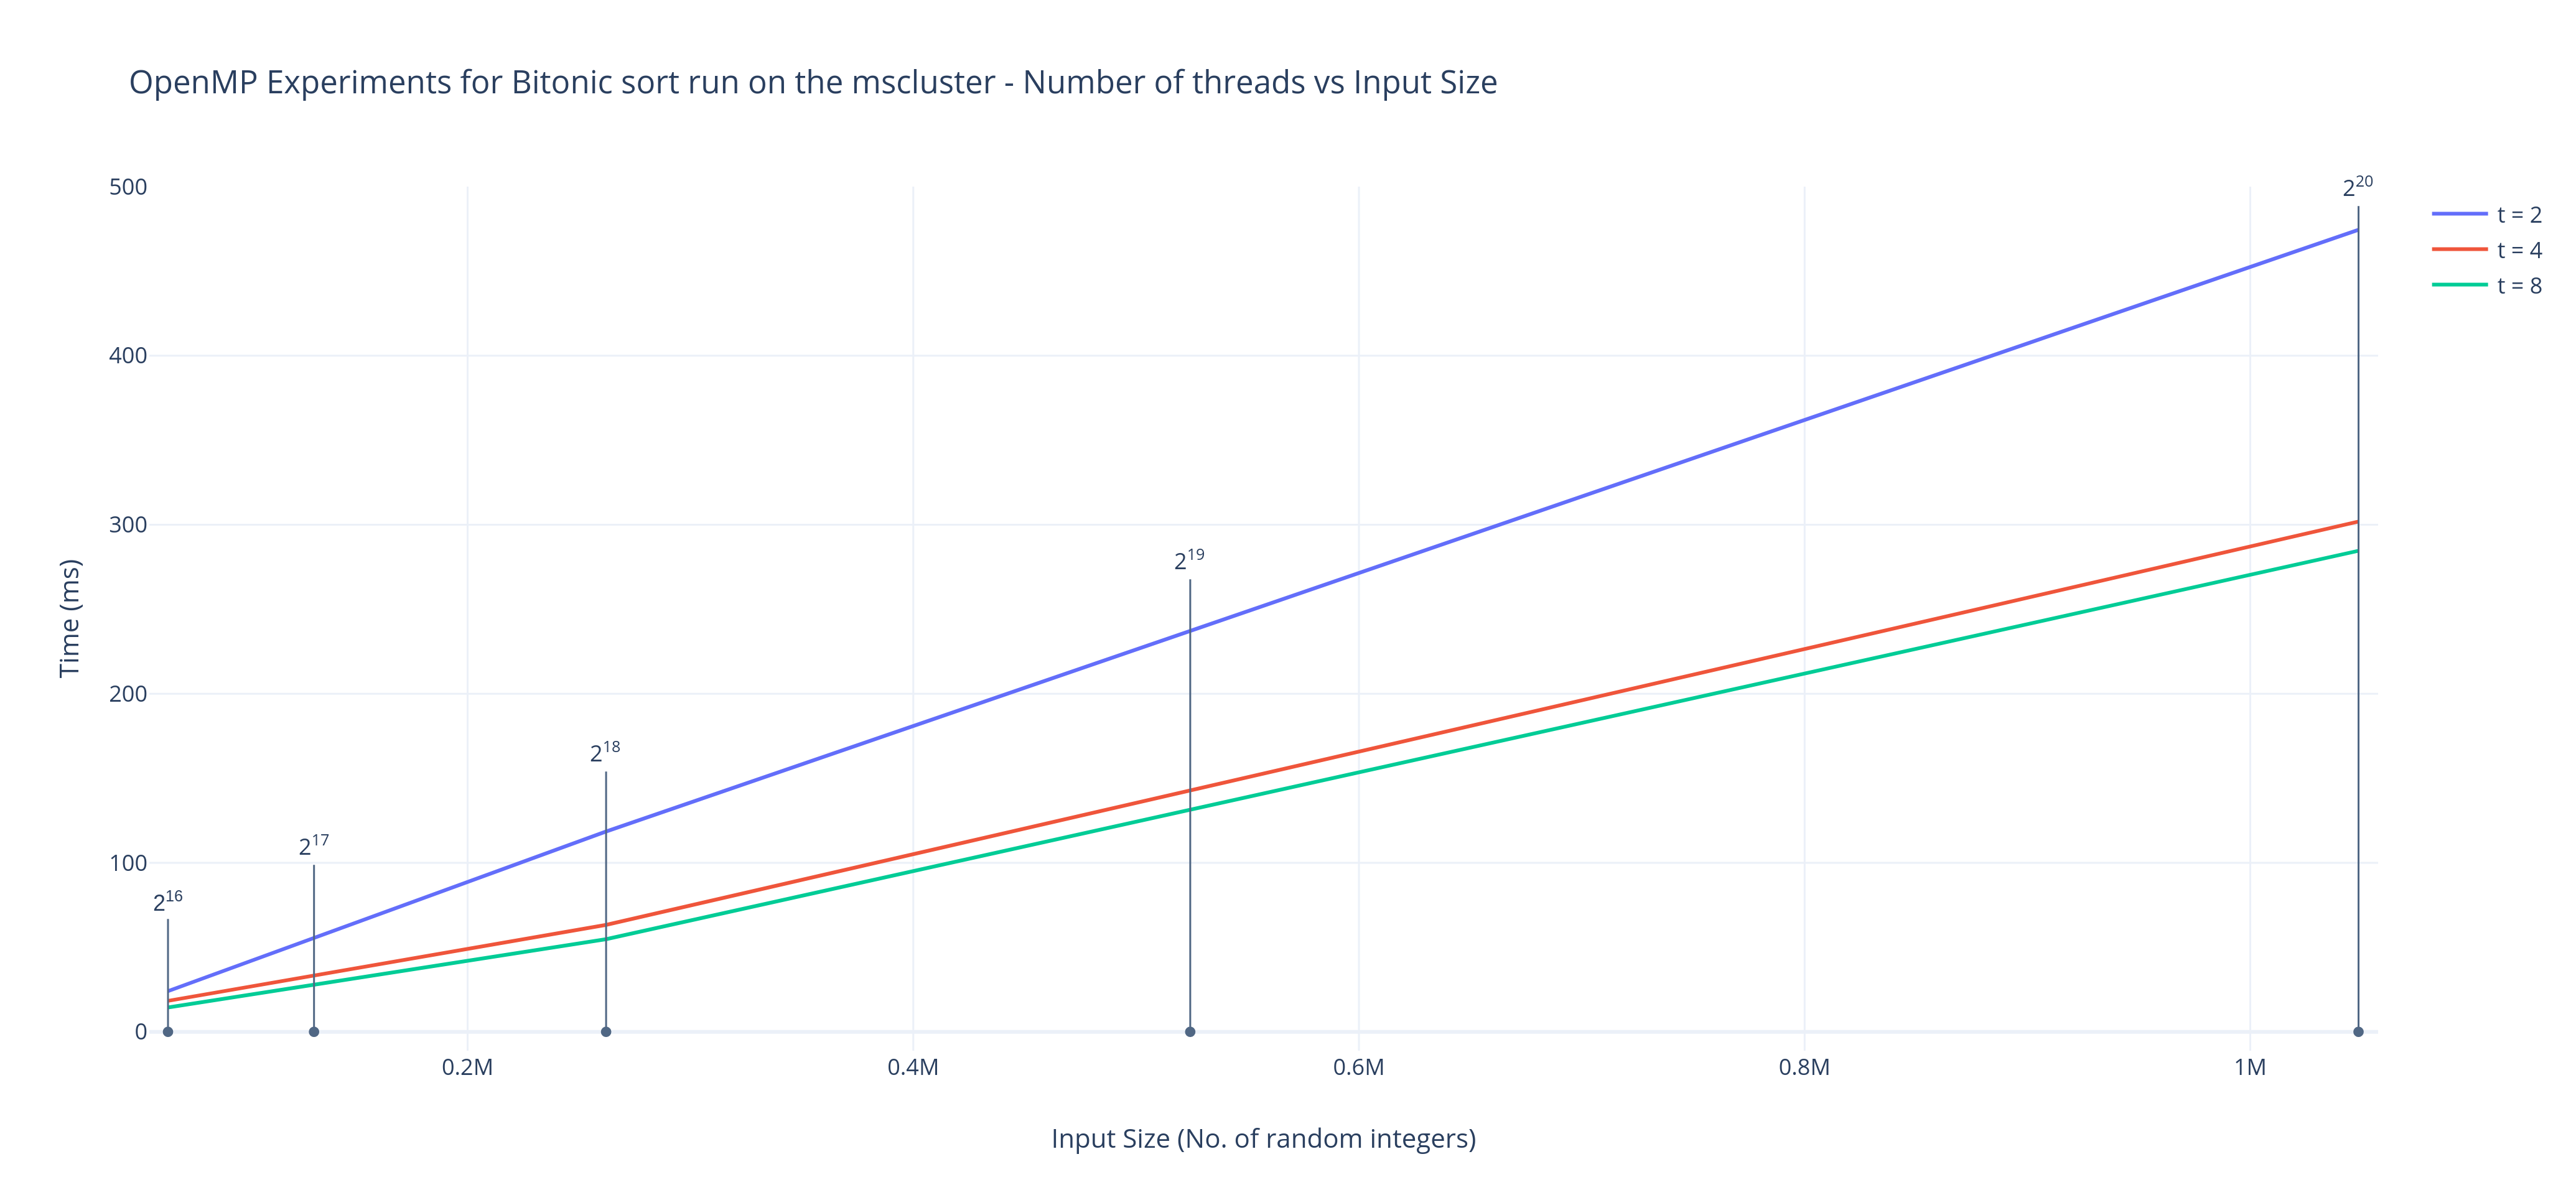
\includegraphics[width=0.8\linewidth]{pics/ompBitonic.png}
    	\caption{OpenMP Comparisons for bitonic sort}\label{fig:ompBitonic}
\end{figure}

From the graph, we can see a direct relation to increasing the number of threads for different input sizes results in a speedup, and that speedup gets significantly better as the input size grows.

\subsection{MPI Implementation}
\textbf{Approach:}

The MPI (Message Passing Interface) implementation aims to parallelize the bitonic sort algorithm by using a distributed computing approach. Unlike the serial and OpenMP versions, which utilized shared memory and threads within a single machine, the MPI implementation utilizes multiple processes running on different machines or nodes within a cluster. Each process has its own memory space and executes a portion of the sorting algorithm independently. The processes communicate with each other by passing messages to exchange data and perform collective operations.

\textbf{Parallelization Methods:}

\begin{enumerate}
\item \textbf{Process Initialization:} The MPI library is initialized using the \lstinline{MPI_Init} function, which assigns a unique rank to each process and determines the total number of processes in the MPI communicator. The \lstinline{MPI_Comm_rank} and \lstinline{MPI_Comm_size} functions are used to obtain the rank and size of the MPI communicator, respectively.

\item \textbf{Data Distribution:} The input data is divided among the processes using the \lstinline{MPI_Scatter} function. The root process broadcasts the entire input array to all other processes using the \lstinline{MPI_Bcast} function. Each process receives a portion of the input array, which it will independently sort.

\item \textbf{Bitonic Sort:} Each process performs the bitonic sort algorithm on its local portion of the array using the \lstinline{bitonic_sort} function. The local sorting is similar to the serial version, where each process sorts its portion of the array independently. This step is performed in parallel by all processes.

\item \textbf{Bitonic Merge:} After the local sorting is completed, the processes perform a bitonic merge operation using the \lstinline{bitonic_merge} function. The merge operation is similar to the serial and OpenMP versions, where elements from different processes are compared and exchanged to create a globally sorted array. This step is performed in parallel by all processes.

\item \textbf{Data Gathering:} The sorted subarrays from each process are gathered and merged by the root process using the \lstinline{MPI_Gather} function. The root process receives the sorted subarrays from all other processes and merges them into a single globally sorted array.
\end{enumerate}

\textbf{Correctness and Testing Methods:}

To ensure the correctness of the MPI implementation, similar testing methods as the serial and OpenMP versions can be employed.

By conducting these testing methods, the correctness of the MPI implementation can be thoroughly evaluated, and any issues or bugs can be identified and addressed. It is crucial to ensure that the parallel code produces accurate results while achieving improved performance in a distributed computing environment.

\subsection{Performance Evaluation}

\subsection*{Comparison of Performance (Speedup) - Serial vs. OpenMP}

To compare the performance between the baseline (serial) and parallel versions of the code, we can calculate the speedup. Speedup measures the improvement in execution time achieved by parallelization compared to the serial version. The following table shows the execution times for the serial and parallel versions, along with the calculated speedup:

\begin{table}[htbp]
  \caption{Comparison of Performance (Speedup) - Serial vs. OpenMP}
  \centering
  \begin{tabular}{lcc}
    \toprule
    \textbf{Description} & \textbf{Time (ms)} & \textbf{Speedup} \\
    \midrule
    Serial Time & 1020.11 ms & -- \\
    Parallel Time & 252.126 ms & 4.04 \\
    \bottomrule
  \end{tabular}
\end{table}

The speedup is calculated as the ratio of the serial time to the parallel time:

\[
\text{Speedup (Serial vs. Parallel)} = \frac{\text{Serial Time}}{\text{Parallel Time}} = \frac{1020.11 \text{ ms}}{252.126 \text{ ms}} = 4.04
\]

This indicates that the parallel version is approximately 4.04 times faster than the serial version.

\subsection*{Comparison of Performance (Speedup) - Serial vs. MPI Version}

Similarly, we can compare the performance between the serial version and the MPI version with 4 processing elements. The following table presents the execution times and speedup for this comparison:

\begin{table}[htbp]
  \caption{Comparison of Performance (Speedup) - Serial vs. MPI Version}
  \centering
  \begin{tabular}{lcc}
    \toprule
    \textbf{Description} & \textbf{Time (ms)} & \textbf{Speedup} \\
    \midrule
    Serial Time & 1020.11 ms & -- \\
    MPI Time (np=4) & 152.6 ms & 6.68 \\
    \bottomrule
  \end{tabular}
\end{table}

The speedup is calculated as the ratio of the serial time to the MPI time:

\[
\text{Speedup (Serial vs. MPI)} = \frac{\text{Serial Time}}{\text{MPI Time (np=4)}} = \frac{1020.11 \text{ ms}}{152.6 \text{ ms}} = 6.68
\]

This indicates that the MPI \cite{mpi} version achieves approximately 6.68 times better performance than the serial version.

\subsection*{Testing Scalability - Varying the Input Size or Number of Processing Elements}

To test the scalability of the algorithm, the input size or the number of processing elements can be varied.

Scalability refers to the ability of a parallel algorithm to maintain or improve its performance as the problem size or the number of processing elements increases. In this case, the scalability can be evaluated by analyzing the execution times for different input sizes while keeping the number of processing elements constant (e.g., np=4).

The following table shows the execution times for different input sizes:

\begin{table}[htbp]
  \centering
  \begin{tabular}{lcc}
    \toprule
    \textbf{Description} & \textbf{Time (ms)} & \textbf{Speedup} \\
    \midrule
    $2^{16}$ & 19.375 ms & 2.40 \\
    $2^{18}$ & 47.6291 ms &  4.62 \\
    $2^{20}$ & 152.6 ms ms  ms &  6.68 \\
    \bottomrule
  \end{tabular}
\end{table}

In summary, the performance evaluation reveals that the parallel version of the code achieves significant speedup compared to the serial version. Additionally, the MPI version with 4 processing elements achieves even better speedup. The algorithm demonstrates scalability as the input size increases, resulting in reduced execution times.

\subsection{Graph Comparison - MPI}
To further evaluate scalability, additional measurements can be taken by varying the input size and analyzing the execution times for different input sizes and number of processing elements. This can help determine if the code scales efficiently as the problem size or resources increase

\begin{figure}[htb]
	\centering
	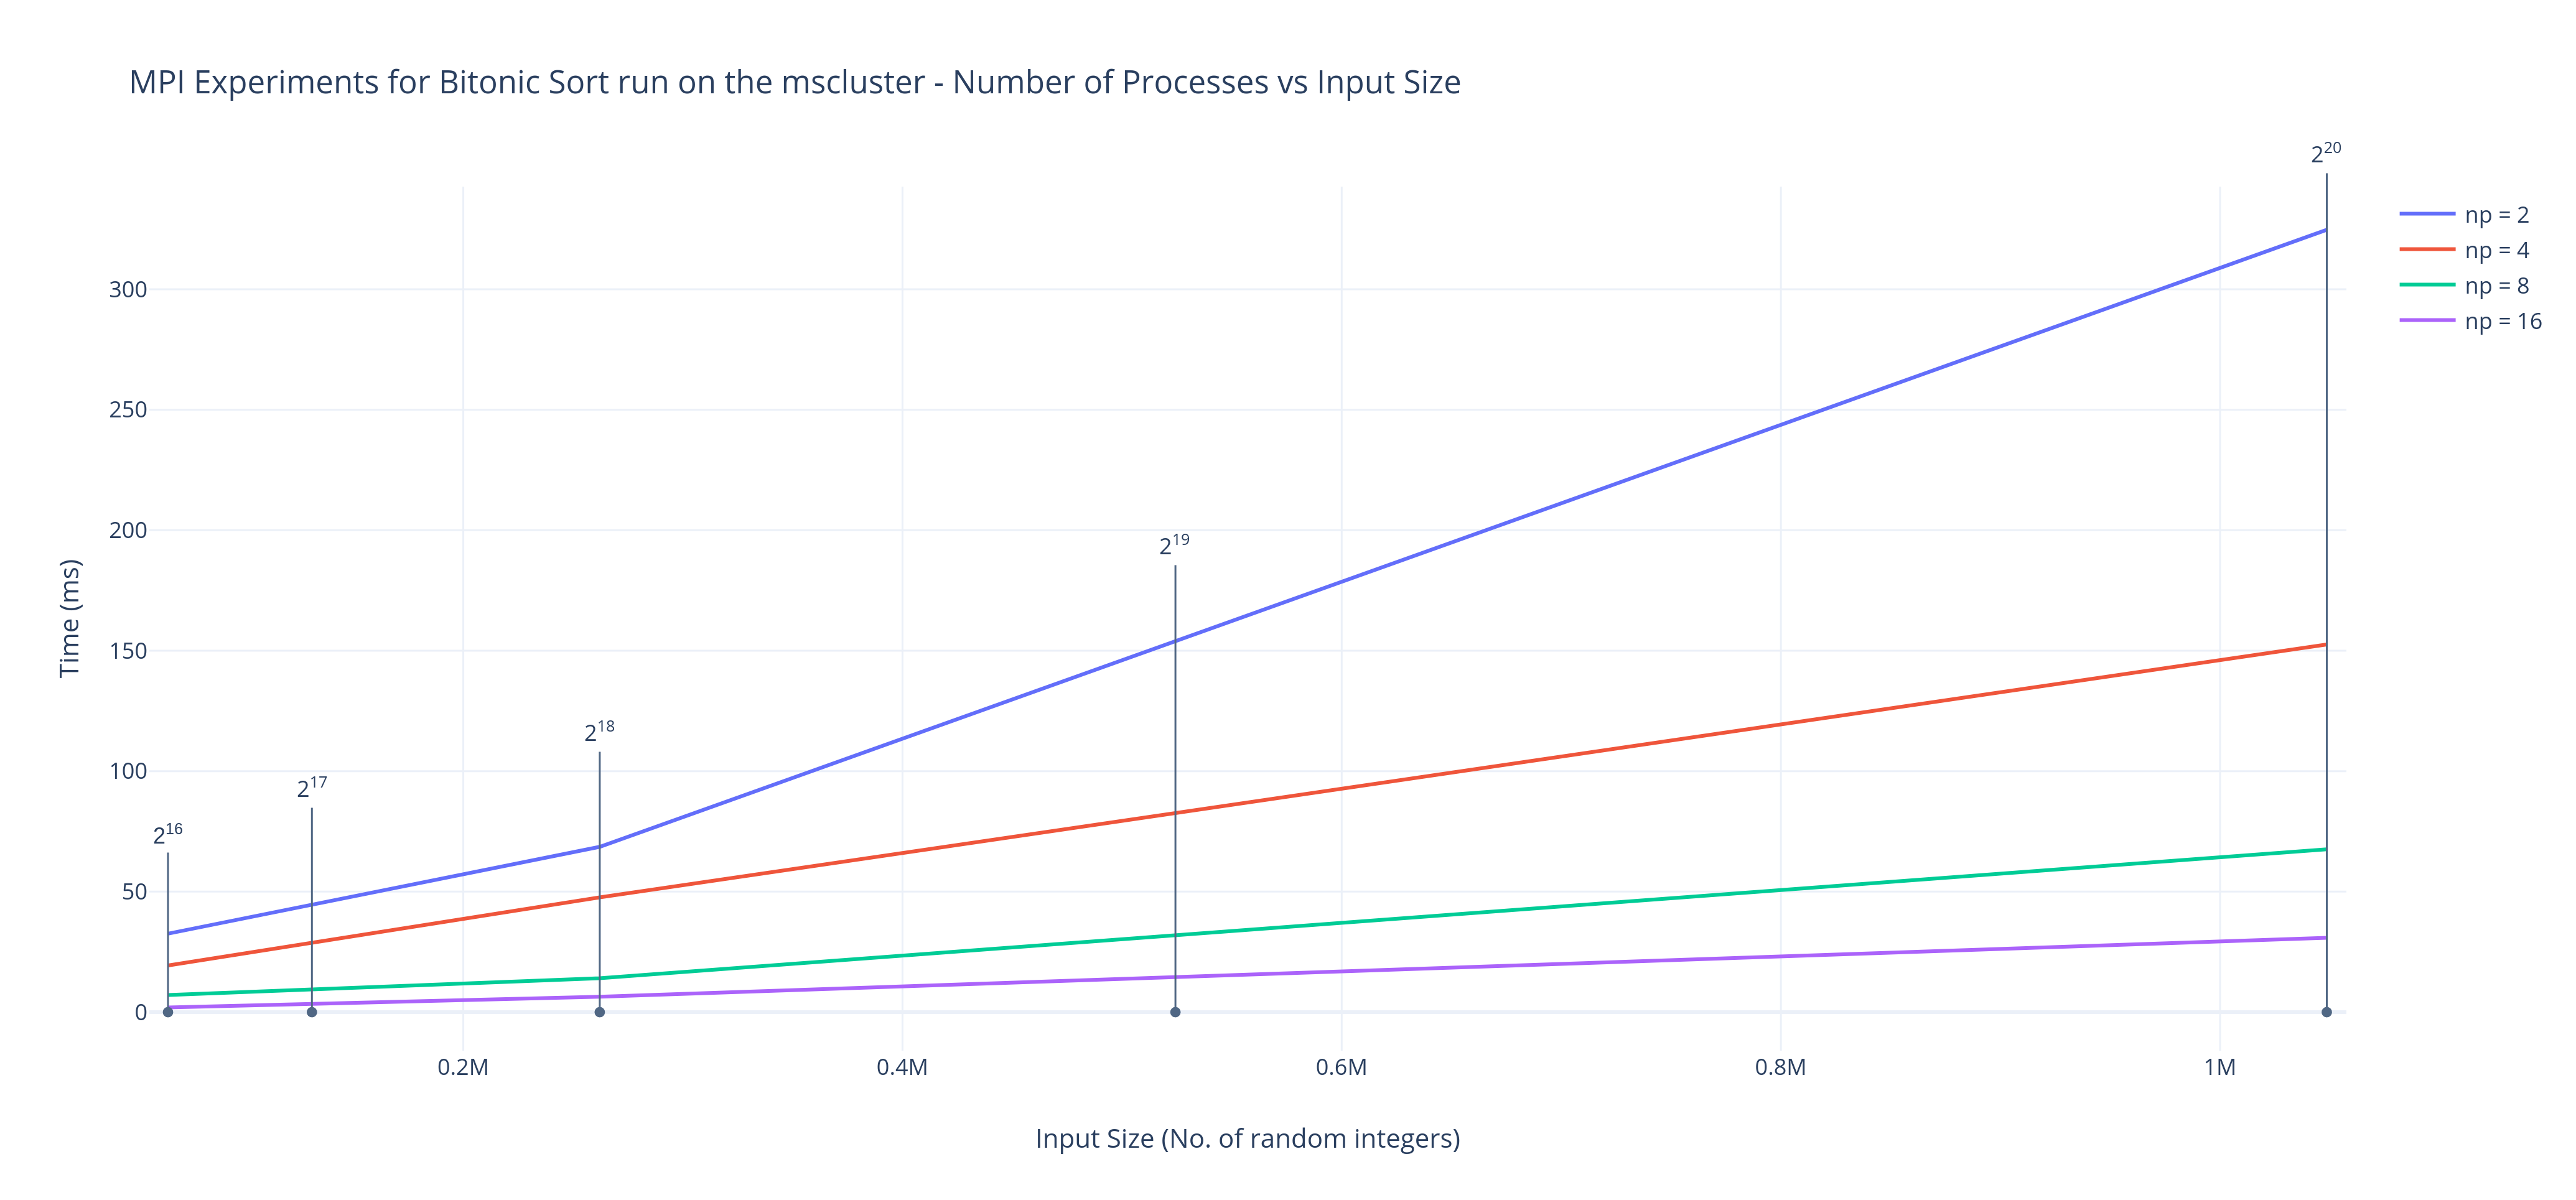
\includegraphics[width=0.9\linewidth]{pics/MPIGraph.png}
    	\caption{MPI Comparisons for bitonic sort}\label{fig:MPIGraph}
\end{figure}

From the graph, we can see a direct relation to increasing the number of processes for different input sizes results in a speedup, and that speedup gets significantly better as the input size grows.

\newpage

\section{Conclusion}
Using OpenMP \cite{openmp} and MPI \cite{openmpmpi} can significantly improve the performance of parallel algorithms like scan and bitonic sort compared to their serial counterparts. By leveraging multiple threads or processes, these parallel programming models allow for efficient utilization of modern multi-core processors and distributed computing systems.

OpenMP enables parallelism at the thread level, where the computation is divided among multiple threads that execute concurrently. By using OpenMP directives, such as parallel for loops or task-based parallelism, the workload can be distributed across threads, leading to improved execution times. Adjusting the number of threads in OpenMP allows for fine-grained control over the level of parallelism and can result in noticeable speed-ups.

On the other hand, MPI allows for parallelism at the process level, enabling computations to be distributed across multiple nodes in a distributed memory system. With MPI, data is explicitly exchanged between processes, facilitating efficient communication and coordination. By carefully orchestrating the communication patterns and workload distribution, significant speed-ups can be achieved in parallel algorithms.

When applying OpenMP and MPI to scan and bitonic sort algorithms, the speed-up is consistently observed by increasing the number of threads or processes. As the workload is divided among more computational units, the overall computation time decreases due to parallel execution and efficient resource utilization. By effectively balancing the workload and minimizing communication overhead, OpenMP and MPI allow for scalability, enabling larger problem sizes to be tackled efficiently.

In conclusion, the combination of OpenMP and MPI, along with adjusting the number of threads or processes, offers a powerful approach to improve the performance of parallel algorithms like scan and bitonic sort. Leveraging the parallelism provided by these programming models can lead to significant speed-ups, enabling efficient processing of large-scale data and computationally intensive tasks.

\newpage

\bibliographystyle{plain}
\bibliography{references}

\end{document} 
